%! Author = Val
%! Date = 2022. 10. 20.

%! Author = Valentinusz
%! Date = 2022. 10. 19.

\documentclass[a4paper,12pt]{article}

\usepackage[margin=1in]{geometry}

\usepackage[utf8]{inputenc}
\usepackage{exsheets}
\usepackage{centernot}
\usepackage{listings}

\DeclareInstance{exsheets-heading}{block-no-nr}{default}{
    attach = {
        main[l,vc]title[l,vc](0pt,0pt) ;
        main[r,vc]points[l,vc](\marginparsep,0pt)
    }
}

\RenewQuSolPair
{question}[headings=runin]
{solution}[headings=block-no-nr]

\SetupExSheets{
    counter-format=qu.,
    solution/print=true ,
    question/name=Feladat,
    solution/name=Megoldás.
}

\usepackage{tasks}
\usepackage[hungarian]{babel}
\usepackage{amsmath}
\usepackage{mathtools}
\usepackage{amsthm}
\usepackage[shortlabels]{enumitem}
\usepackage{amsfonts}
\usepackage{amssymb}
\usepackage{graphicx}
\usepackage{wrapfig}
\graphicspath{{./images/}}
\usepackage{float}
\usepackage{multicol}
\usepackage{tikz}
\usepackage{booktabs}
\usepackage{lstmisc}
\usetikzlibrary{positioning,shapes,fit,arrows}
\tikzset{every picture/.style={line width=0.75pt}} %set default line width to 0.75pt

\title{\huge{Programozáselmélet} \\ \large 5. gyakorlat}
\author{Boda Bálint}
\date{2022. őszi félév}

\theoremstyle{definition}
\newtheorem{definition}{Definíció}
\newtheorem*{definition*}{Definíció}
\newtheorem*{remark}{Megjegyzés}
\newtheorem{theorem}{Tétel}
\newtheorem*{theorem*}{Tétel}
\newtheorem*{example}{Példa}

\DeclareMathOperator{\lf}{lf}
\DeclareMathOperator{\ps}{p(S)}

\SetupExSheets{solution/print=true}
\SetupExSheets{question/name=}
\SetupExSheets{headings=runin}

\begin{document}
    \maketitle
    \begin{definition*}[Paramétertér]
        Azt mondjuk, hogy a $B$ halmaz az $ F \subseteq A \times A $ feladat egy \textbf{paramétertere}, ha
        \[ \exists F_1 \subseteq A \times B, \; F_2 \subseteq B \times A: \quad F = F_2 \circ F_1 \]
    \end{definition*}
    \begin{theorem*}[Specifikáció]
        Legyen $ F \subseteq A \times A $ egy feladat és legyen $B$ $F$ egy paramétertere.
        Legyen $b \in B$ egy tetszőleges paraméter, amihez definiáljuk a $Q_b: A \rightarrow \mathbb{L}$ és
        $R_b: A \rightarrow \mathbb{L}$ logikai függvényeket:
        \begin{align*}
            \lceil Q_b \rceil &\coloneqq F_{1}^{(-1)}(b) \\
            \lceil R_b \rceil &\coloneqq F_{2}(b)
        \end{align*}
        Ekkor, ha $ \forall b \in B: Q_b \implies \lf{(S, R_b)} $, akkor $S$ megoldja az $F$ feladatot.
    \end{theorem*}
    \setcounter{question}{4}
    \begin{question}(4. feladatsor) Legyen $ A = [1..4] $. $ S \subseteq A \times (A \cup {fail})^{**}$ a következő program:
    \[
        S =\left\{
            \begin{array}{ll,2}
                1 \rightarrow \left< 1,2,4,1 \right>, & 1 \rightarrow \left< 1,3,2 \right>,& 2 \rightarrow \left< 2,3 \right>, \\
                3 \rightarrow \left< 3,2 \right>,     & 3 \rightarrow \left< 3,4 \right>, & 4 \rightarrow \left< 4,1,3 \right>
            \end{array}
            \right\}
    \]
    Legyen $ B = \{ x,y,z \} $ az $ F $ feladat egy paramétertere, adott továbbá
    \begin{align*}
        F1 &= \{(1,x), (2,y), (2,z), (3,z), (4,y)\} \\
        F2 &= \{(x,1), (x,2), (y,3), (z,2), (z,4)\}
    \end{align*}
        \begin{tasks}
            \task Adjuk meg az $F$ feladatot elemeinek felsorolásávál!
            \task Mint mond a specifikáció tétele az $S$ programról és az $F$ feladatról?
        \end{tasks}
    \end{question}
    \newpage
    \begin{solution}
        \begin{figure}[H]
            \centering
            \[ F_2 \circ F_1 \]
            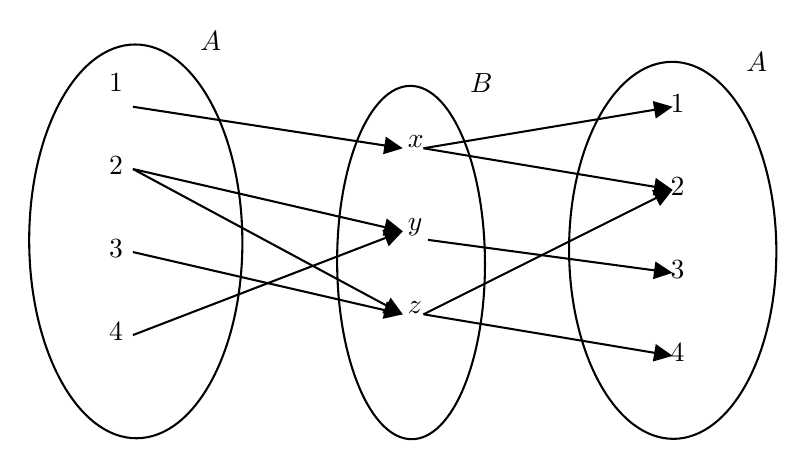
\begin{tikzpicture}[x=0.75pt,y=0.75pt,yscale=-1,xscale=1]

%uncomment if require: \path (0,300); %set diagram left start at 0, and has height of 300

%Shape: Ellipse [id:dp381402362061003]
                \draw   (111.81,249.72) .. controls (83.44,249.85) and (60.26,207.48) .. (60.02,155.09) .. controls (59.79,102.7) and (82.58,60.12) .. (110.94,60) .. controls (139.31,59.87) and (162.49,102.23) .. (162.73,154.62) .. controls (162.96,207.02) and (140.17,249.59) .. (111.81,249.72) -- cycle ;
%Shape: Ellipse [id:dp4090156922606536]
                \draw   (370.48,250) .. controls (342.9,250.12) and (320.36,209.56) .. (320.14,159.4) .. controls (319.91,109.24) and (342.08,68.48) .. (369.66,68.35) .. controls (397.23,68.23) and (419.77,108.79) .. (420,158.95) .. controls (420.23,209.11) and (398.06,249.87) .. (370.48,250) -- cycle ;
%Shape: Ellipse [id:dp857074088444007]
                \draw   (244.39,250.16) .. controls (224.72,250.25) and (208.6,212.22) .. (208.39,165.21) .. controls (208.18,118.21) and (223.95,80.03) .. (243.62,79.94) .. controls (263.28,79.85) and (279.4,117.88) .. (279.61,164.89) .. controls (279.83,211.89) and (264.06,250.07) .. (244.39,250.16) -- cycle ;
%Straight Lines [id:da9302952538618898]
                \draw    (110,90) -- (237.03,109.54) ;
                \draw [shift={(240,110)}, rotate = 188.75] [fill={rgb, 255:red, 0; green, 0; blue, 0 }  ][line width=0.08]  [draw opacity=0] (8.93,-4.29) -- (0,0) -- (8.93,4.29) -- cycle    ;
%Straight Lines [id:da23018262756407948]
                \draw    (110,120) -- (237.08,149.33) ;
                \draw [shift={(240,150)}, rotate = 192.99] [fill={rgb, 255:red, 0; green, 0; blue, 0 }  ][line width=0.08]  [draw opacity=0] (8.93,-4.29) -- (0,0) -- (8.93,4.29) -- cycle    ;
%Straight Lines [id:da8714178759746892]
                \draw    (110,120) -- (237.36,188.58) ;
                \draw [shift={(240,190)}, rotate = 208.3] [fill={rgb, 255:red, 0; green, 0; blue, 0 }  ][line width=0.08]  [draw opacity=0] (8.93,-4.29) -- (0,0) -- (8.93,4.29) -- cycle    ;
%Straight Lines [id:da33526108795849596]
                \draw    (110,160) -- (237.08,189.33) ;
                \draw [shift={(240,190)}, rotate = 192.99] [fill={rgb, 255:red, 0; green, 0; blue, 0 }  ][line width=0.08]  [draw opacity=0] (8.93,-4.29) -- (0,0) -- (8.93,4.29) -- cycle    ;
%Straight Lines [id:da09738902819253803]
                \draw    (110,200) -- (237.2,151.08) ;
                \draw [shift={(240,150)}, rotate = 158.96] [fill={rgb, 255:red, 0; green, 0; blue, 0 }  ][line width=0.08]  [draw opacity=0] (8.93,-4.29) -- (0,0) -- (8.93,4.29) -- cycle    ;
%Straight Lines [id:da1023826248168197]
                \draw    (250,110) -- (367.04,90.49) ;
                \draw [shift={(370,90)}, rotate = 170.54] [fill={rgb, 255:red, 0; green, 0; blue, 0 }  ][line width=0.08]  [draw opacity=0] (8.93,-4.29) -- (0,0) -- (8.93,4.29) -- cycle    ;
%Straight Lines [id:da7001252063718018]
                \draw    (250,110) -- (367.04,129.51) ;
                \draw [shift={(370,130)}, rotate = 189.46] [fill={rgb, 255:red, 0; green, 0; blue, 0 }  ][line width=0.08]  [draw opacity=0] (8.93,-4.29) -- (0,0) -- (8.93,4.29) -- cycle    ;
%Shape: Boxed Line [id:dp9499815170075446]
                \draw    (252.13,154.13) -- (367.03,169.6) ;
                \draw [shift={(370,170)}, rotate = 187.67] [fill={rgb, 255:red, 0; green, 0; blue, 0 }  ][line width=0.08]  [draw opacity=0] (8.93,-4.29) -- (0,0) -- (8.93,4.29) -- cycle    ;
%Straight Lines [id:da05514137698853128]
                \draw    (250,190) -- (367.32,131.34) ;
                \draw [shift={(370,130)}, rotate = 153.43] [fill={rgb, 255:red, 0; green, 0; blue, 0 }  ][line width=0.08]  [draw opacity=0] (8.93,-4.29) -- (0,0) -- (8.93,4.29) -- cycle    ;
%Straight Lines [id:da5614579398280519]
                \draw    (250,190) -- (367.04,209.51) ;
                \draw [shift={(370,210)}, rotate = 189.46] [fill={rgb, 255:red, 0; green, 0; blue, 0 }  ][line width=0.08]  [draw opacity=0] (8.93,-4.29) -- (0,0) -- (8.93,4.29) -- cycle    ;

% Text Node
                \draw (141,52.4) node [anchor=north west][inner sep=0.75pt]    {$A$};
% Text Node
                \draw (404,62.4) node [anchor=north west][inner sep=0.75pt]    {$A$};
% Text Node
                \draw (271,72.4) node [anchor=north west][inner sep=0.75pt]    {$B$};
% Text Node
                \draw (97,72.4) node [anchor=north west][inner sep=0.75pt]    {$1$};
% Text Node
                \draw (97,112.4) node [anchor=north west][inner sep=0.75pt]    {$2$};
% Text Node
                \draw (97,152.4) node [anchor=north west][inner sep=0.75pt]    {$3$};
% Text Node
                \draw (97,192.4) node [anchor=north west][inner sep=0.75pt]    {$4$};
% Text Node
                \draw (241,102.4) node [anchor=north west][inner sep=0.75pt]    {$x$};
% Text Node
                \draw (241,142.4) node [anchor=north west][inner sep=0.75pt]    {$y$};
% Text Node
                \draw (241,182.4) node [anchor=north west][inner sep=0.75pt]    {$z$};
% Text Node
                \draw (367.55,82.63) node [anchor=north west][inner sep=0.75pt]    {$1$};
% Text Node
                \draw (367.55,122.63) node [anchor=north west][inner sep=0.75pt]    {$2$};
% Text Node
                \draw (367.55,162.63) node [anchor=north west][inner sep=0.75pt]    {$3$};
% Text Node
                \draw (367.55,202.63) node [anchor=north west][inner sep=0.75pt]    {$4$};
            \end{tikzpicture}\label{fig:figure}
        \end{figure}

        \begin{tasks}
            \task $F = \left\{ (1,1), (1,2), (2,2), (2,3), (2,4), (3,2), (3,4), (4,3) \right\}$

            \begin{array}{ll,1}

            \end{array}
            \task{$ \ps(1) = \{1,2\},\quad \ps(2) = \{3\},\quad \ps(3) = \{2,4\},\quad \ps(4) = \{3\} \\ \forall b \in \{x,y,z\}:  $
            \begin{enumerate}
                \item{$ b = x$ \checkmark
                    \begin{align*}
                        \lceil Q_x \rceil = F_1^{(-1)}(x) &= \{1\} \\
                        \lceil R_x \rceil = F_2(x) &= \{1,2\} \\
                        \lf{(S,R_x)} &= \{ a \in \{1,2,3,4\}\;|\;a \in \{1,2,3,4\} \; \land \; \ps(a) \subseteq \{1,2\} \} = \{1\}
                    \end{align*} $ \lceil Q_x \rceil \implies \lf{(S,R_x)} $, mert $ \{1\} \subseteq \{1\} $}
                \item{$ b = y$ \checkmark
                    \begin{align*}
                        \lceil Q_y \rceil = F_1^{(-1)}(y) &= \{2,4\} \\
                        \lceil R_y \rceil = F_2(y) &= \{3\} \\
                        \lf{(S,R_y)} &= \{ a \in \{1,2,3,4\}\;|\;a \in \{1,2,3,4\} \; \land \; \ps(a) \subseteq \{3\} \} = \{2,4\}
                    \end{align*} $ \lceil Q_y \rceil \implies \lf{(S,R_y)} $, mert $ \{2,4\} \subseteq \{2,4\} $}
                \item{$ b = z $ \xmark
                    \begin{align*}
                        \lceil Q_z \rceil = F_1^{(-1)}(z) &= \{2,3\} \\
                        \lceil R_z \rceil = F_2(z) &= \{2,4\} \\
                        \lf{(S,R_y)} &= \{ a \in \{1,2,3,4\}\;|\;a \in \{1,2,3,4\} \; \land \; \ps(a) \subseteq \{2,4\} \} = \{3\}
                    \end{align*} $ \lceil Q_y \rceil \centernot \implies \lf{(S,R_y)} $, mert $ \{2,3\} \not \subseteq \{3\} $}
            \end{enumerate}}
        \end{tasks}
        A specifikáció tétele ezen esetben nem mond semmit.
        Annak megállapítása, hogy $S$ megoldja-e az $F$ feladatot, további vizsgálatot igényel.
    \end{solution}
    \newpage
    \setcounter{question}{2}
    \begin{question}(5. feladatsor)
        Adott az $F$ feladat specifikációja:
        \begin{align*}
            A &= (x: \mathbb{Z}, y: \mathbb{Z}, z: \mathbb{Z}) \\
            B &= (x': \mathbb{Z}, y': \mathbb{Z}) \\
            Q &= (x = x' \; \land \; y = y' \; \land \; x' > 5) \\
            R &= (Q \; \land \; x > y \rightarrow z = x)
        \end{align*}
        \begin{tasks}
            \task Adjuk meg a $Q_{\{x':4, y':2\}}: A \rightarrow \mathbb{L} $ függvény igazsághalmazát!
            \task Mit rendel $F$ az állapottér $ \{ x:4,y:2,z:1 \} $, $ \{ x:8,y:5,z:7 \} $, $ \{ x:9,y:3,z:10 \} $, $ \{ x:6,y:9,z:4 \} $ elemeihez?
        \end{tasks}
    \end{question}
    \begin{solution}
        \begin{remark}
            Az implikáció igazságtáblázata a következő:
            \begin{table}[H]
                \centering
                \begin{tabular}{llc}
                    \textbf{$p$} & \textbf{$q$} & \textbf{$p \implies q$} \\
                    $I$ & $I$ & $I$ \\
                    $I$ & $H$ & $H$ \\
                    $H$ & $I$ & $I$ \\
                    $H$ & $H$ & $I$ \\
                \end{tabular}
                \label{tab:}
            \end{table}
        \end{remark}
        \begin{figure}[H]
            \centering
            \label{fig:figure2}
            \tikzset{every picture/.style={line width=0.75pt}} %set default line width to 0.75pt
            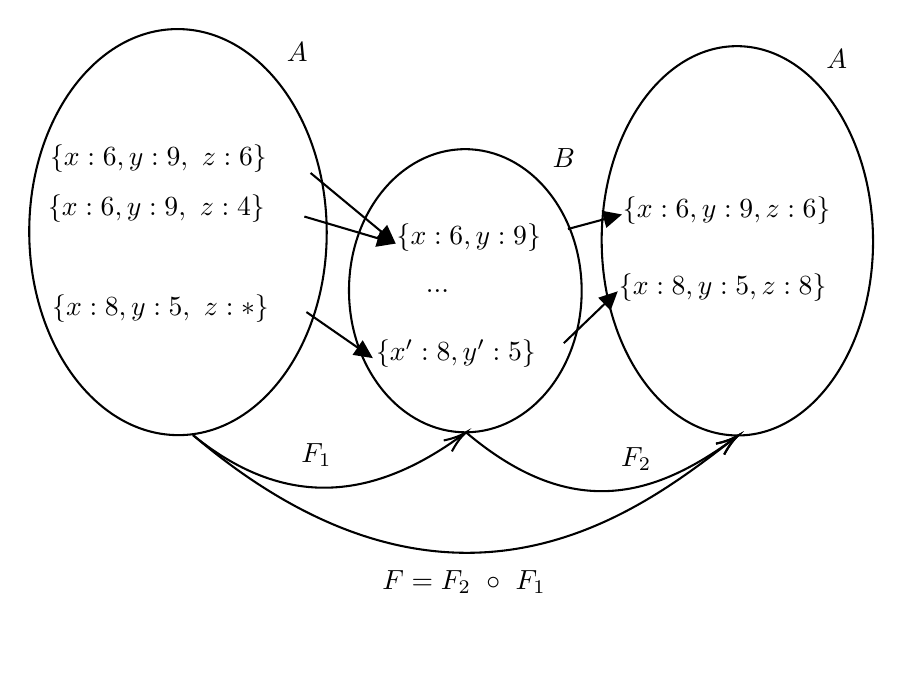
\begin{tikzpicture}[x=0.75pt,y=0.75pt,yscale=-1,xscale=1]
%uncomment if require: \path (0,395); %set diagram left start at 0, and has height of 395

%Shape: Ellipse [id:dp381402362061003]
                \draw   (104.49,250.81) .. controls (64.91,250.99) and (32.62,207.34) .. (32.38,153.32) .. controls (32.13,99.29) and (64.02,55.35) .. (103.6,55.17) .. controls (143.18,55) and (175.47,98.64) .. (175.71,152.67) .. controls (175.96,206.69) and (144.07,250.63) .. (104.49,250.81) -- cycle ;
%Shape: Ellipse [id:dp4090156922606536]
                \draw   (373.98,250.97) .. controls (337.87,251.14) and (308.41,209.28) .. (308.18,157.49) .. controls (307.94,105.69) and (337.02,63.57) .. (373.13,63.4) .. controls (409.23,63.24) and (438.69,105.1) .. (438.93,156.89) .. controls (439.16,208.69) and (410.08,250.81) .. (373.98,250.97) -- cycle ;
%Shape: Ellipse [id:dp857074088444007]
                \draw   (242.8,249.45) .. controls (211.84,249.59) and (186.61,219.16) .. (186.44,181.49) .. controls (186.27,143.82) and (211.22,113.17) .. (242.18,113.03) .. controls (273.13,112.89) and (298.37,143.31) .. (298.54,180.98) .. controls (298.71,218.65) and (273.75,249.31) .. (242.8,249.45) -- cycle ;
%Straight Lines [id:da5370138954545506]
                \draw    (165.93,191.5) -- (195.47,211.99) ;
                \draw [shift={(197.93,213.7)}, rotate = 214.75] [fill={rgb, 255:red, 0; green, 0; blue, 0 }  ][line width=0.08]  [draw opacity=0] (8.93,-4.29) -- (0,0) -- (8.93,4.29) -- cycle    ;
%Curve Lines [id:da9242147906610455]
                \draw    (111.26,250.78) .. controls (158.46,289.31) and (201.92,279.65) .. (241.6,250.34) ;
                \draw [shift={(242.8,249.45)}, rotate = 143.13] [color={rgb, 255:red, 0; green, 0; blue, 0 }  ][line width=0.75]    (10.93,-3.29) .. controls (6.95,-1.4) and (3.31,-0.3) .. (0,0) .. controls (3.31,0.3) and (6.95,1.4) .. (10.93,3.29)   ;
%Curve Lines [id:da6104497322332579]
                \draw    (242.8,249.45) .. controls (293.42,292.27) and (333.18,281.2) .. (372.78,251.87) ;
                \draw [shift={(373.98,250.97)}, rotate = 143.13] [color={rgb, 255:red, 0; green, 0; blue, 0 }  ][line width=0.75]    (10.93,-3.29) .. controls (6.95,-1.4) and (3.31,-0.3) .. (0,0) .. controls (3.31,0.3) and (6.95,1.4) .. (10.93,3.29)   ;
%Curve Lines [id:da8944242148823418]
                \draw    (111.26,250.78) .. controls (240.63,360.59) and (332.13,282.57) .. (372.76,251.89) ;
                \draw [shift={(373.98,250.97)}, rotate = 143.13] [color={rgb, 255:red, 0; green, 0; blue, 0 }  ][line width=0.75]    (10.93,-3.29) .. controls (6.95,-1.4) and (3.31,-0.3) .. (0,0) .. controls (3.31,0.3) and (6.95,1.4) .. (10.93,3.29)   ;
%Straight Lines [id:da9910581971902204]
                \draw    (164.93,145.5) -- (206.06,157.65) ;
                \draw [shift={(208.93,158.5)}, rotate = 196.46] [fill={rgb, 255:red, 0; green, 0; blue, 0 }  ][line width=0.08]  [draw opacity=0] (8.93,-4.29) -- (0,0) -- (8.93,4.29) -- cycle    ;
%Straight Lines [id:da43684451784834255]
                \draw    (291.93,151.5) -- (315.04,145.28) ;
                \draw [shift={(317.93,144.5)}, rotate = 164.93] [fill={rgb, 255:red, 0; green, 0; blue, 0 }  ][line width=0.08]  [draw opacity=0] (8.93,-4.29) -- (0,0) -- (8.93,4.29) -- cycle    ;
%Straight Lines [id:da5872741560104443]
                \draw    (167.93,124.5) -- (206.62,156.58) ;
                \draw [shift={(208.93,158.5)}, rotate = 219.67] [fill={rgb, 255:red, 0; green, 0; blue, 0 }  ][line width=0.08]  [draw opacity=0] (8.93,-4.29) -- (0,0) -- (8.93,4.29) -- cycle    ;
%Straight Lines [id:da3371503684356998]
                \draw    (289.93,206.5) -- (313.77,183.58) ;
                \draw [shift={(315.93,181.5)}, rotate = 136.12] [fill={rgb, 255:red, 0; green, 0; blue, 0 }  ][line width=0.08]  [draw opacity=0] (8.93,-4.29) -- (0,0) -- (8.93,4.29) -- cycle    ;

% Text Node
                \draw (155,60.4) node [anchor=north west][inner sep=0.75pt]    {$A$};
% Text Node
                \draw (415,63.4) node [anchor=north west][inner sep=0.75pt]    {$A$};
% Text Node
                \draw (283,111.4) node [anchor=north west][inner sep=0.75pt]    {$B$};
% Text Node
                \draw (198,203.4) node [anchor=north west][inner sep=0.75pt]    {$\{x':8,y':5\}$};
% Text Node
                \draw (41.93,181.57) node [anchor=north west][inner sep=0.75pt]    {$\{x:8,y:5,\ z:*\}$};
% Text Node
                \draw (39.93,133.57) node [anchor=north west][inner sep=0.75pt]    {$\{x:6,y:9,\ z:4\}$};
% Text Node
                \draw (207.93,147.57) node [anchor=north west][inner sep=0.75pt]    {$\{x:6,y:9\}$};
% Text Node
                \draw (315,171.4) node [anchor=north west][inner sep=0.75pt]    {$\{x:8,y:5,z:8\}$};
% Text Node
                \draw (162,253.4) node [anchor=north west][inner sep=0.75pt]    {$F_{1}$};
% Text Node
                \draw (316,255.4) node [anchor=north west][inner sep=0.75pt]    {$F_{2}$};
% Text Node
                \draw (201,314.4) node [anchor=north west][inner sep=0.75pt]    {$F=F_{2} \ \circ \ F_{1}$};
% Text Node
                \draw (222,179.4) node [anchor=north west][inner sep=0.75pt]    {$...$};
% Text Node
                \draw (316.93,134.57) node [anchor=north west][inner sep=0.75pt]    {$\{x:6,y:9,z:6\}$};
% Text Node
                \draw (40.93,109.57) node [anchor=north west][inner sep=0.75pt]    {$\{x:6,y:9,\ z:6\}$};


            \end{tikzpicture}

        \end{figure}
        \begin{tasks}
            \task $ \lceil Q_{\{x':4,y':2\}} \rceil = F_1^{(-1)}(\{x':4,y':2\}) = \{ a \in A \; | \; x(a) = 4 \; \land \; y(a) = 2 \; \land \; 4>5 \} = \{\} $
            \task
            \begin{align*}
                F(\{ x:4,y:2,z:1 \}) &= \{\} \\
                F(\{ x:8,y:5,z:7 \}) &= \{a \in A \; | x(a) = 8 \; \land \; y(a) = 5 \; \land \; 8 > 5 \; \land \; 8 > 5 \implies x(a) = z(a) \} \\ &= {\{x:8,y:5,z:8}\} \\
                F(\{ x:9,y:3,z:10 \}) &= {\{x:9,y:3,z:9}\} \\
                F(\{ x:6,y:9,z:4 \}) &= \{a \in A \; | x(a) = 6 \; \land \; y(a) = 9 \; \land \; 6 > 5 \; \land \; 6 > 9 \implies x(a) = z(a) \} \\ &= {\{a \in A \; | \; x(a) = 6 \; \land \; y(a) = 9 \}}
            \end{align*}
        \end{tasks}
    \end{solution}
    \setcounter{question}{1}
    \begin{question}
        Adott az $F$ feladat specifikációja:
        \begin{align*}
            A &= (x: \mathbb{Z}, y: \mathbb{Z}, z: \mathbb{Z}) \\
            B &= (x': \mathbb{Z}, y': \mathbb{Z}) \\
            Q &= (x = x' \; \land \; y = y') \\
            R &= ((z = x' \; \lor \; z = y') \; \land \; z \ge x' \; \land \; z \ge y')
        \end{align*}
        \begin{tasks}
            \task Adjuk meg a $ Q_{\{x':6,y':5\}}: A \rightarrow \mathbb{L} $ függvény igazsághalmazát.
            \task Adjuk meg a $ R_{\{x':6,y':5\}}: A \rightarrow \mathbb{L} $ függvény igazsághalmazát.
            \task Mit rendel $F$ az $ {\{x:6,y:5, z:3\}} $ állapothoz?
        \end{tasks}
    \end{question}
    \begin{solution}
        \begin{tasks}
            \task $ \lceil Q_{\{x':6,y':5\}} \rceil = F_1^{(-1)}(\{x':6,y':5\}) = \{ a \in A \; | \; x(a) = 6 \; \land \; y(a) = 5 \} $
            \task Figyeljük meg hogy a feladat utófeltétele nem követeli meg, hogy az előfeltétel igaz maradjon,
            azaz a kezdőállapot $x$ és $y$ változói megváltozhatnak. \\
            $ \lceil R_{\{x':6,y':5\}} \rceil = \{\{x:a,y:b,z:6 \; | \; a,b \in \mathbb{Z}\}\} $
            \task A kérdést a b feladat megválaszolta.
        \end{tasks}
    \end{solution}
\end{document}